%! Author = wolfram_e_laube
%! Date = 06.05.24

\item[(a)]
\section*{Task (a): Spectrum of \(x(t)\)}

\subsection*{Problem Statement}
The analog signal defined by
\[
x(t) = \sin(2\pi f_1 t) + \sin(2\pi f_2 t)
\]
where \(f_1 = 4000\) kHz and \(f_2 = 6000\) kHz, is analyzed to determine its frequency spectrum.

\subsection*{Theoretical Background}
The Fourier Transform of a continuous signal provides a representation of its frequency content.
For a sine wave, the transform results in delta functions located at the frequencies of the sine components,
reflecting the concentration of energy at those frequencies.

\subsection*{Mathematical Derivation}
Using the Fourier Transform, the spectrum of \(x(t)\) is derived as:
\[
X(f) = \pi \left(\delta(f - 4000) - \delta(f + 4000) + \delta(f - 6000) - \delta(f + 6000)\right) / i
\]
This shows that the signal comprises frequency components at \(\pm 4000\) Hz and \(\pm 6000\) Hz.

\subsection*{Python Implementation and Plot}
The frequency spectrum of \(x(t)\) was visualized using Python, clearly showing the delta spikes at the aforementioned frequencies.
The plot Figure~\ref{fig:spectrum} below illustrates these components.

\begin{figure}[h]
    \centering
    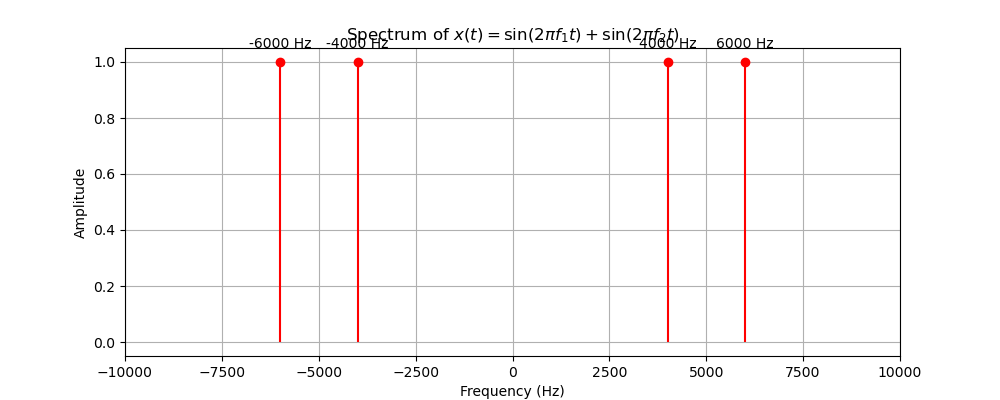
\includegraphics[width=0.8\textwidth]{fig/ex1_a_spectrum}
    \caption{Spectrum of \(x(t)\) showing delta spikes at \(\pm 4000\) Hz and \(\pm 6000\) Hz.}
    \label{fig:spectrum}
\end{figure}

\subsection*{Conclusion}
The analysis confirms the presence of significant frequency components at \(\pm 4000\) Hz and \(\pm 6000\) Hz in the signal \(x(t)\).